Das Ziel bei der Kommunikation zwischen zwei oder mehreren Geräten ist es, dass diese trotz Unterschiedlicher Hersteller und verschiedenen Technologien problemlos miteinander kommunizieren können. Um das zu erreichen, wurde das OSI-Referenzmodell (Open System Interconnection) entwickelt, welches die Kommunikation in 7 Teilaufgaben zerlegt, die als hierarchische Schichten (\emph{layers}) dargestellt werden können.
\begin{figure}[H]
\centering
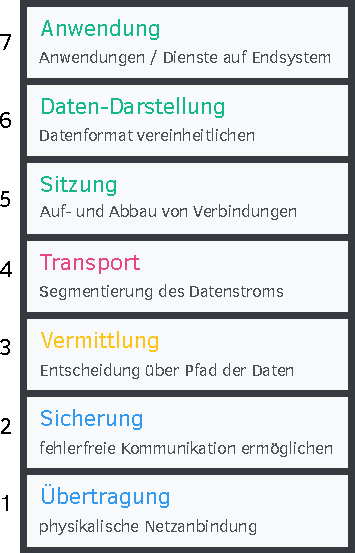
\includegraphics[width=0.382\textwidth]{graphics/a2.pdf}
\caption{Aufbau des OSI-Schichtenmodells mit (stark) vereinfachten Beschreibungen}
\end{figure}

\subsubsection{Schicht 1: Übertragung}
Die Übertragungsschicht (engl. \emph{physical layer}) beschreibt als unterste Ebene im OSI-Modell die physikalische Netzanbindung, d.h. die Umsetzung der Daten (Bits) in die messbare/empfangbare physikalische Größe und deren Form, also leitungsgebunden, Funkübertragung oder Lichtwellenübertragung, sowie Modulationsart und auch Kabel, Verbinder etc.

\subsubsection{Schicht 2: Sicherungsschicht}
Aufgabe der Sicherrungsschicht (engl. \emph{data-link layer}) ist die gewährleistung einer zuverlässigen, möglichst fehlerfreien Kommunikation. Sie regelt den Zugriff auf das Übertragungsmedium (Schicht 1) und führt Maßnahmen zu Flusskontrolle sowie Fehlerkontrolle durch Prüfsummen/Kanalkodierung durch. In dieser Schicht werden die Daten in \emph{Frames} eingeteilt (z.B. Ethernet-Frames (siehe \ref{A4.6}).
Schicht 2 wird unterteilt in \emph{LLC} und \emph{MAC}:
\begin{enumerate}
        \item[2b)] LLC, Logical Link Control\\
        \small Schnittstelle zwischen Layer 3 und MAC
        \item[2a)] MAC, Media Access Control\\
        \small regelt zugriff auf gemeinsames Medium
\end{enumerate}

\subsubsection{Schicht 3: Vermittlungs- / Netzwerkschicht}
Die Vermittlungsschicht (engl. \emph{network layer}) ist dafür zuständig, die Daten \emph{blockweise}, d.h. als sog. \emph{Pakete} zwischen den Endsystemen weiterzuvermitteln. Außerdem ist sie für die Stauvermeidung (Congestion Control), sowie die Wegsuche zwischen den Zwischensystemen / Netzwerkknoten (Routing) zuständig. Schicht 3 stellt weiterhin Netzwerkadressen bereit (z.B. IP), aktualisiert Routing-Tabellen und fragmentiert die Datenpakete.

\subsubsection{Schicht 4: Transportschicht}
In der Transportschicht (engl. \emph{transport layer}) wird der Datenstrom segmentiert, d.h. aufgeteilt auf mehrere Pakete (je nach Maximum Segment Size (MSS)), wobei jedem ein Header angefügt wird, welcher u.a. die Segmente nummeriert und das zugrundeliegende Protokoll (z.B. TCP oder UDP) sowie Ziel- und Quellport kennzeichnet. Mit Ziel und Quellport werden hier den segmentierten Datenpaketen Anwendungen auf den Endsystemen zugewiesen.

\subsubsection{Schicht 5: Sitzungsschicht}
Die Sitzungsschicht (engl. \emph{session layer}), auch Kommunikationsschicht, regelt den Auf- u. Abbau von Kommunikationssitzungen und ermöglicht die Wiederherstellung dieser nach Abbrüchen (Synchronisation).

\subsubsection{Schicht 6: Präsentationsschicht}
Die Präsentationsschicht (engl. \emph{presentation layer}) setzt die systemabhängige Darstellung der Daten (z.B. \textsc{ASCII}, \textsc{EBCDIC}) in eine unabhängige Form um, um den Datenaustausch zwischen unterschiedlichen Systemen zu ermöglichen. Außerdem fallen Aufgaben wie Datenkompression und -verschlüsselung in diese Ebene.

\subsubsection{Schicht 7: Applikationsschicht}
In der Anwendungsschicht befinden sich die Dienste der Anwendungsprogramme auf den jeweiligen Endsystemen. Hier findet man Protokolle wie HTTP, DNS, SMTP, FTP etc. Die Anwendungsprogramme selbst gehören nicht dazu.

